%%%%%%%%%%%%%%%%%%%%%%%%%%%%%%%%%%%%%
\part{Preliminaries}
%%%%%%%%%%%%%%%%%%%%%%%%%%%%%%%%%%%%%

%%% --------------------------
\section{Motivation}
%%% --------------------------
\normalfont
\begin{frame}
	\begin{center}
  		\begin{alertblock}{Motivation} 
  			\begin{itemize}
  				\item Derive and convey key insights from data
  				\item Learn and use open source software
  				\item Explore first/another programming language
  				\item Gain ability to create insightful visualizations
  				\item Be more marketable 
  			\end{itemize}
		\end{alertblock}

	       \begin{center}
	         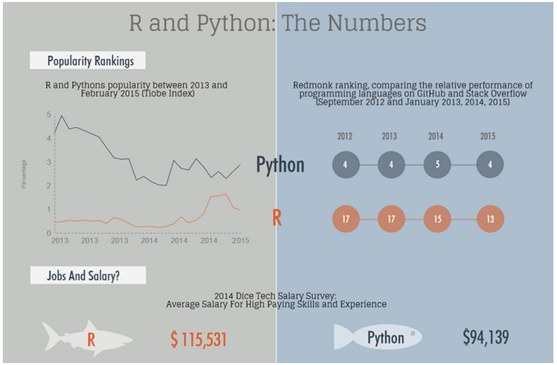
\includegraphics[scale=0.25]{images/r-vs-python-numbers}[6]
	        \end{center}

	\end{center} 
\end{frame}


\normalfont
\begin{frame}
	\begin{center}
  		\begin{block}{Disclaimer} 
The author assumes you are:
	\begin{itemize}
		\item \itshape not \normalfont familiar with \ttfamily R \normalfont 
		\item \itshape need not \normalfont have programmed before
		\item \itshape are \normalfont interested in working with data 
		\item \itshape are \normalfont curious how to best convey findings
	\end{itemize} 
	\end{block}

	       \begin{center}
	         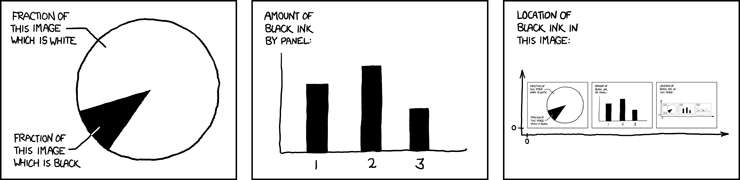
\includegraphics[scale=0.35]{images/xkcd-self_description}[8]
	        \end{center}

	\end{center} 
\end{frame}

%%% --------------------------
\section{Why R?}
%%% --------------------------
\begin{frame}
	\begin{center}
  		\begin{block}{Why R?} 
			\begin{itemize}
				\item Absolutely free!
				\item Used in industry and academia.
				\item Has a great community:
					\begin{itemize}
						\item StackOverflow
						\item Blogs
						\item Meetup groups
						\item MOOCs
						\item many, many others
					\end{itemize}
				\item Has over 7500 packages available for use (for free!).
				\item Transparent code (e.g. easier to check for bugs).
			\end{itemize}
		\end{block}
	\end{center} 
\end{frame}

%%% --------------------------
\section{Why visualize?}
%%% --------------------------
\begin{frame}
	\begin{center}
  		\begin{block}{Why visualize?} 
			\begin{itemize}
				\item \small Capture uncertainty in the data
				\item Explore potential relationships/trends/missing patterns (or absence thereof)
				\item Convey key information \normalfont
			\end{itemize}		
		\end{block}
	\end{center} 

   \begin{center}
     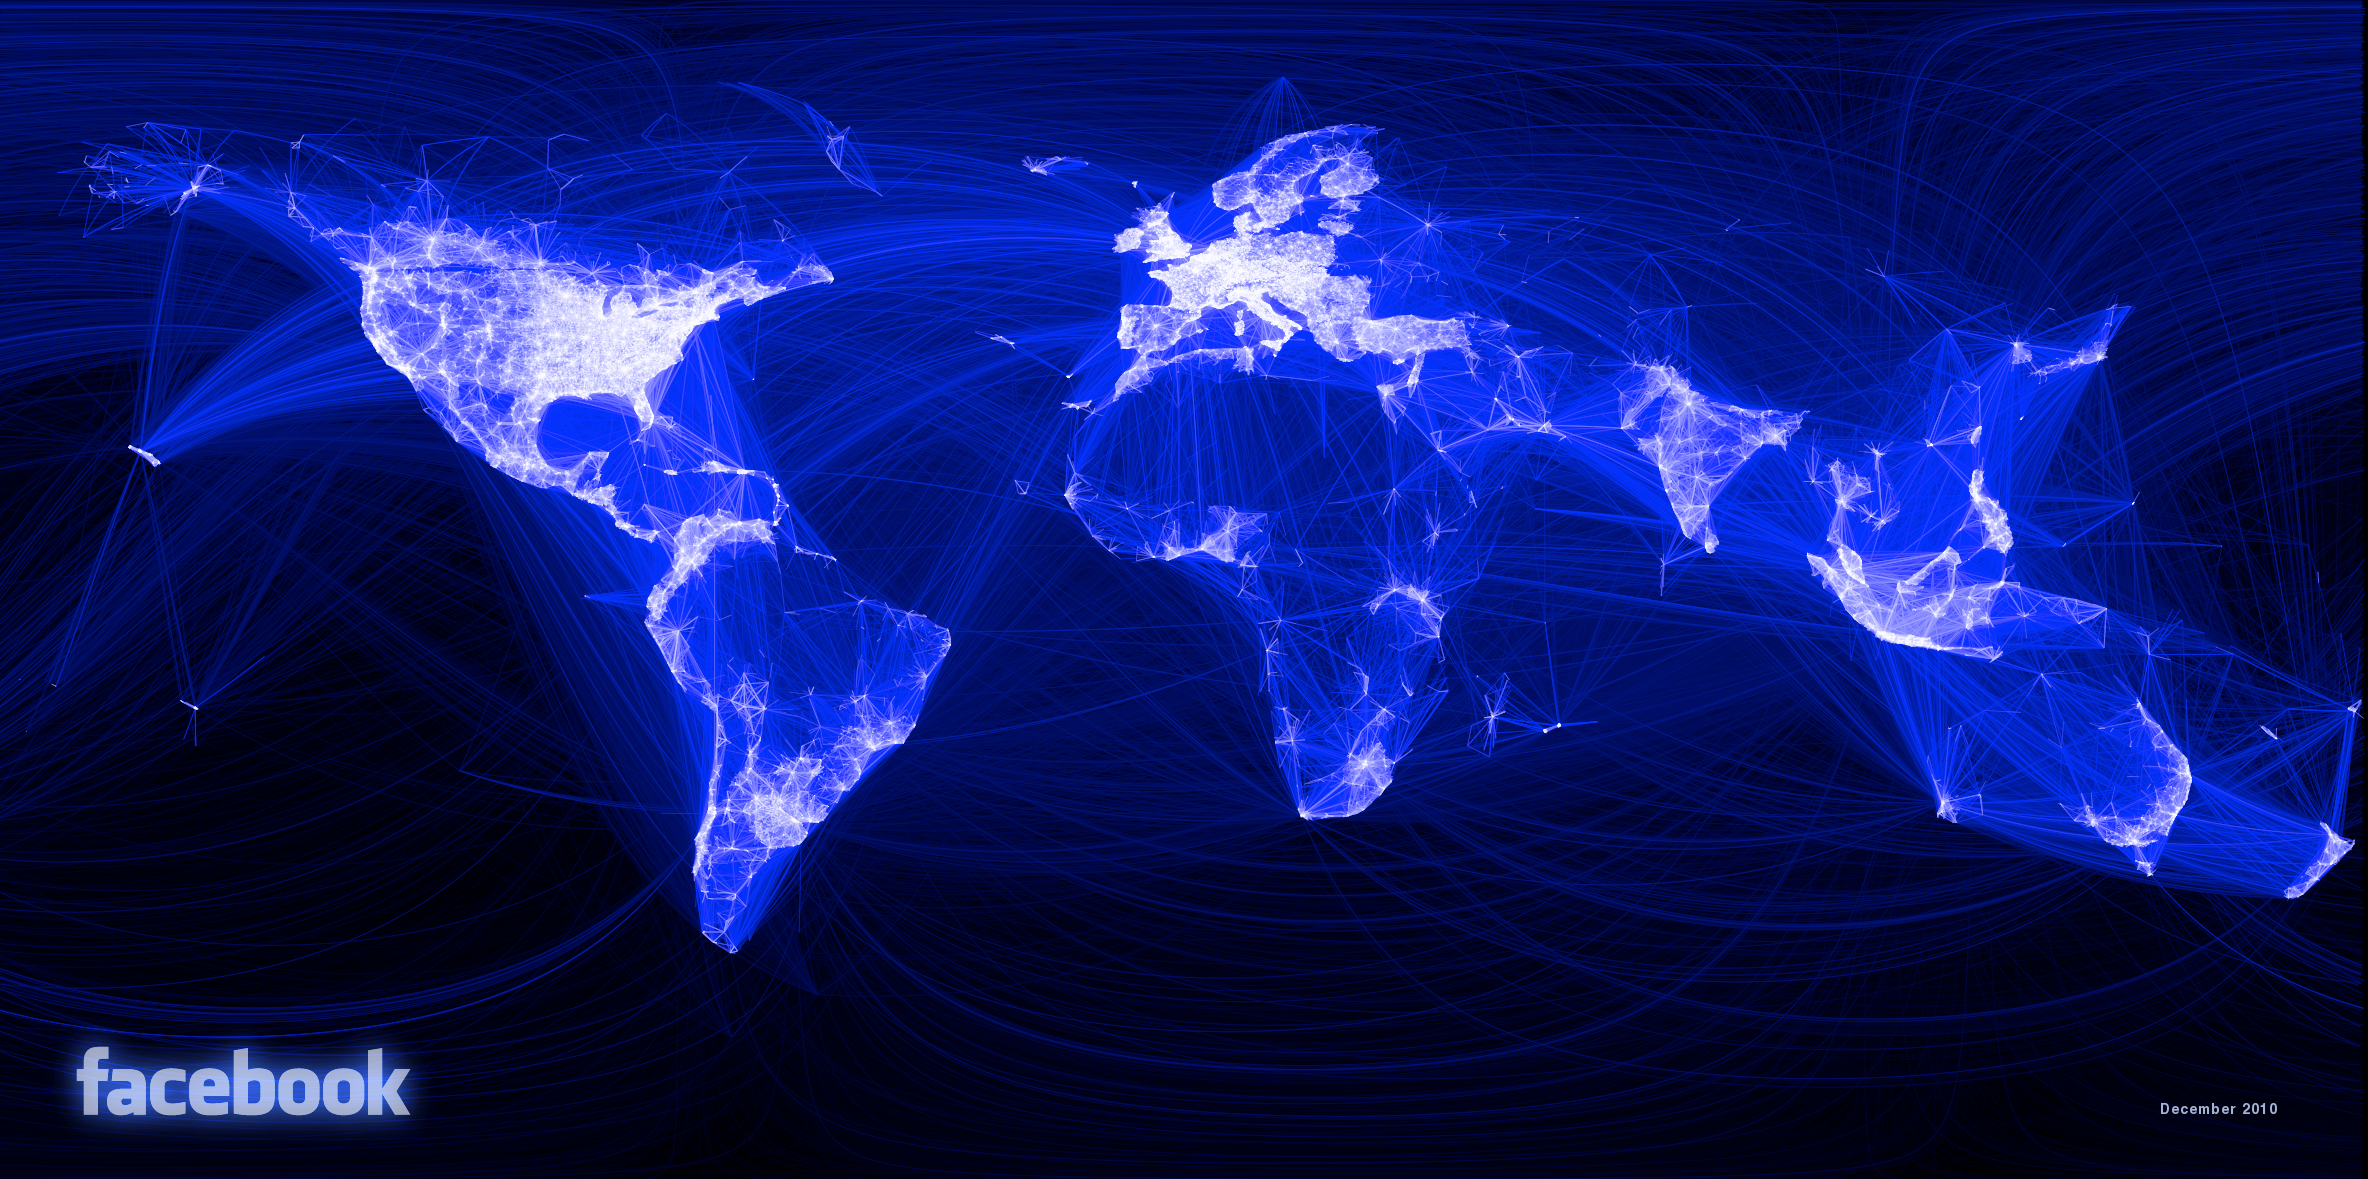
\includegraphics[scale=0.09]{images/facebook}[8]
    \end{center}

\end{frame}
%---

%%% --------------------------
\section{Tips for Visulizations}
%%% --------------------------
\begin{frame}
	\begin{center}
  		\begin{block}{Tips for visualizations} 
			\begin{itemize}
				\item Know your audience 
				\item \itshape{ 15 second rule:} \normalfont if your audience won't be able to understand the graphic in 15 seconds, simplify
				\item Color and font choices
				\item Add text/labels to figure
			\end{itemize}		
		\end{block}
	\end{center} 

  \begin{center}
  	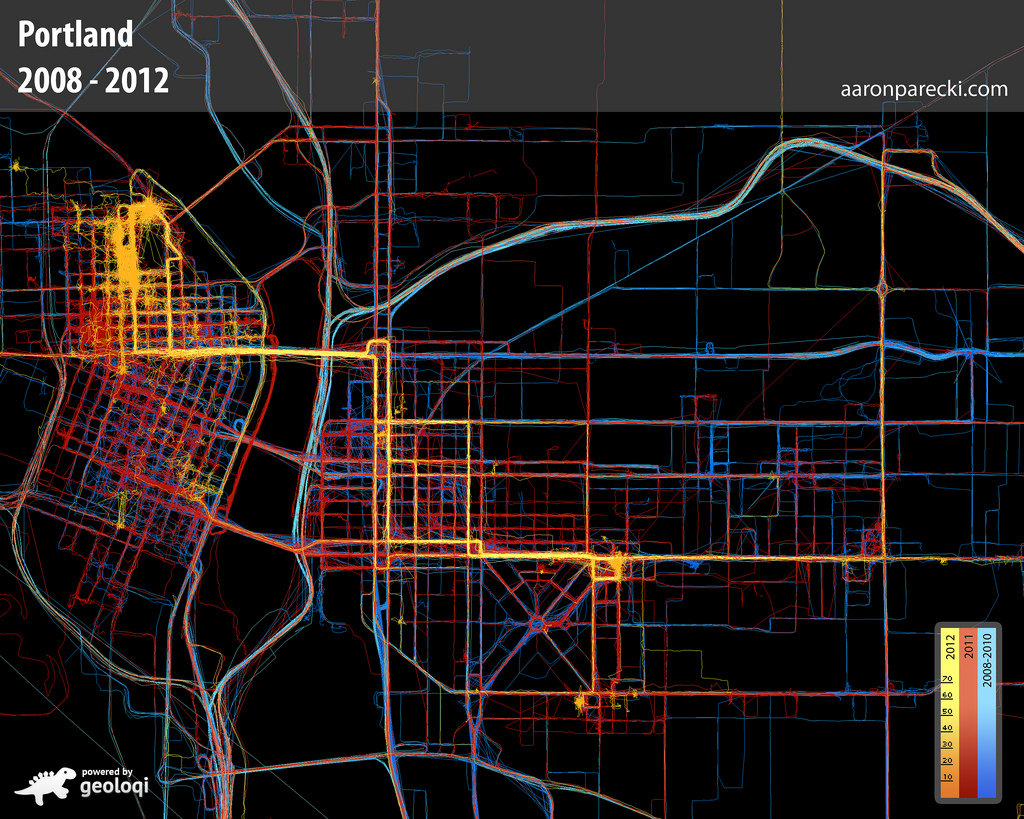
\includegraphics[width=0.4\textwidth]{images/geolocation_ex}[7]
  \end{center}

\end{frame}
%---

%%%%%%%%%%%%%%%%%%%%%%%%%%%%%%%%%%%%%
\part{Introduction to R}
%%%%%%%%%%%%%%%%%%%%%%%%%%%%%%%%%%%%%

%%% --------------------------
\section{Overview of R}
%%% --------------------------
\begin{frame}
	\begin{center}
  		\begin{block}{Overview of R per John Chambers [1]:} 
			"To understand computations in R, two slogans are helpful:
			\begin{itemize}
			        \item Everything that exists is an object.
			        \item Everything that happens is a function call."
			\end{itemize}
		\end{block}
	\end{center} 

% R is flexible: 
% 	\begin{itemize}
% 		\item Objects can be variables, data sets, etc. and can be self-created, downloaded off the web (or elsewhere) and loaded from package(s).
% 		\item Functions (which do something to objects) can also be self-created, downloaded off the web (or elsewhere) and loaded from package(s).
% 		\item A package (1 of 7500+) is a collection of data sets and/or functions unified with a common theme.
% 	\end{itemize}
\end{frame}

%----
%%% --------------------------
\section[Data Types]{Most Common Data Types}
%%% --------------------------
\begin{frame}[fragile]
	\frametitle{Most Common Data Types in R}
	\framesubtitle{Vectors}

	\begin{itemize}
		\item[vector:] contains observations of the same type (e.g. all numbers, letters)
			\begin{itemize}
				\item e.g. movie ratings (on scale 0-10) of the last movie that 5 people saw
				\begin{lstlisting}
c(8,7,10,3,9)
				\end{lstlisting} 
				\begin{verbatim}
[1]  8  7 10  3  9
				\end{verbatim}				
			\end{itemize}
	\end{itemize}
\end{frame}

%---
\begin{frame}[fragile]
	\frametitle{Most Common Data Types in R}
	\framesubtitle{Lists}

	\begin{itemize}
		\item[list:] contains observations of (same or) different types and (same or) different lengths
			\begin{itemize}
				\item e.g. movie ratings of each movie that 5 people saw last month 
			\end{itemize}
		\end{itemize}

   \begin{columns}
     \column{0.5\textwidth}
		\begin{lstlisting}
list(
	c(8,NA,8),
	c(7,7,3),
	10,
	c(3,4,4,NA),
	c(9,10,9,2)
	)
		\end{lstlisting}

     \column{0.5\textwidth}
      \begin{center}
{ \tiny
				\begin{verbatim} 
[[1]]
[1]  8 NA  8

[[2]]
[1] 7 7 3

[[3]]
[1] 10

[[4]]
[1]  3  4  4 NA

[[5]]
[1]  9 10  9  2
			\end{verbatim} \normalsize
}
       \end{center}
     \end{columns}

\end{frame}

%---
\begin{frame}[fragile]
	\frametitle{Most Common Data Types in R}
	\framesubtitle{Matrices}

	\begin{itemize}
		\item[matix:] has rows and columns of numbers
			\begin{itemize}
				\item e.g. movie ratings of 5 people of last 3 movies that each person saw 
			\end{itemize}
		\end{itemize}

   \begin{columns}
     \column{0.45\textwidth}
     	\begin{center}
		\begin{lstlisting}[ basicstyle=\tiny]
	matrix(
	  c(
	    8,NA,8,
	    7,7,3,
		3,4,4,
		9,10,9,
		10,10,9
		),
	  nrow=5,
	  ncol=3,
	  byrow=TRUE
	  )
		\end{lstlisting}
     	\end{center}
     \column{0.45\textwidth}
      \begin{center}
{ \small
				\begin{verbatim} 
     [,1] [,2] [,3]
[1,]    8   NA    8
[2,]    7    7    3
[3,]    3    4    4
[4,]    9   10    9
[5,]   10   10    9
			\end{verbatim} \normalsize
}
       \end{center}
     \end{columns}
\end{frame}


%---
\begin{frame}[fragile]
	\frametitle{Most Common Data Types in R}
	\framesubtitle{Data Frames}

	\begin{itemize}
		\item[$\quad \quad \quad \quad \quad \quad \quad \quad \quad$ data.frame:]
	\end{itemize}

\end{frame}

%%% --------------------------
\section[Assignment]{Creating Objects}
%%% --------------------------
\begin{frame}
	\begin{center}
		\begin{block}{Creating objects in R}

		\end{block}
	\end{center} 
\end{frame}


%%% --------------------------
\section[Functions]{Functions}
\subsection{(Very) Brief Overview of Functions}
%%% --------------------------
\begin{frame}[fragile]
	\begin{center}
		\begin{block}{Function by example}
			\begin{lstlisting}[ basicstyle=\tiny]
f <- function(x, y=1){
	answer <- x * 2 + y + 1
	return(answer)
}

f(2)        # 6
f(3, 2)     # 9
f(y=3, 2)   # 8
f(y=3, x=3) # 10
			\end{lstlisting}	
		\end{block}

		\begin{block}{Components of a function:}
			\begin{itemize}
				\item Assign the function to a variable
				\item Add the 'function' keyword
				\item Specify any arguments (if any) that the function needs to compute the result
				\item Specify any argument defaults
			\end{itemize}
					%%% Assignment, arguments, named, order, unamed
		\end{block}
	\end{center} 
\end{frame}

%%% --------------------------
\subsection{Adding Functionality to Base R}
%%% --------------------------

\begin{frame}
	\begin{center}
			%%% What is base R?
	\end{center} 
\end{frame}



%%%%%%%%%%%%%%%%%%%%%%%%%%%%%%%%%%%%%%

%%%%%%%%%%%%%%%%%%%%%%%%%%%%%%%%%%%%%%


%%%%%%%%%%%%%%%%%%%%%%%%%%%%%%%%%%%%%

% Subsection: Importing Data Sets into R

\section[Importing Data]{Importing Data Sets into R}

% Data Available in R
\subsection{Using Data Available in R}

%%%%%%%%%%%%%%%%%%%%%%%%%%%%%%%%%%%%%
\begin{frame}[fragile]
 \frametitle{Using Data Available in R}
\begin{enumerate}
\item To use a data set available in one of the R packages, install that package (if needed).

\item Load the package into R, using the \ttfamily library() \normalfont function. \\
	\begin{lstlisting}
library(alr3)
	\end{lstlisting}

\item Extract the data set you want from that package, using the \ttfamily data() \normalfont function.  
	\begin{lstlisting}
data(UN2)
	\end{lstlisting}

\end{enumerate}
\end{frame}

% Data Available in R
\subsection{Importing Data from a Previous R Session}

%%%%%%%%%%%%%%%%%%%%%%%%%%%%%%%%%%%%%
\begin{frame}[fragile]
 \frametitle{Importing Data from a Previous R Session}

\end{frame}


%%% Subsection: Importing Data from the Internet

\subsection{Importing Data from the Internet}

%%%%%%%%%%%%%%%%%%%%%%%%%%%%%%%%%%%%%
% --------------------------------------------------- Slide --
\begin{frame}[fragile]
 \frametitle{Data from the Internet}

When downloading data from the internet, use \ttfamily read.table(). \normalfont  In the arguments of the function:
  \begin{itemize}
  \item \ttfamily header: \normalfont if TRUE, tells R to include variables names when importing
  \item \ttfamily sep: \normalfont tells R how the entires in the data set are separated
    \begin{itemize}
      \item \ttfamily sep=",": \normalfont when entries are separated by COMMAS
      \item \ttfamily sep="$\backslash t$": \normalfont when entries are separated by TAB
      \item \ttfamily sep=" ": \normalfont when entries are separated by SPACE
    \end{itemize}
   \end{itemize}
   	\begin{lstlisting}[ basicstyle=\small]
data <- read.table(
	file="http://www.ats.ucla.edu/stat/data/binary.csv", 
	header=TRUE, 
	sep=","
	)
	\end{lstlisting}
\normalfont
\normalsize
\end{frame}

%%%%%%%%%%%%%%%%%%%%%%%%%%%%%%%%%%%%%

% Data from your Computer

\subsection{Importing Data from Your Computer}

%%%%%%%%%%%%%%%%%%%%%%%%%%%%%%%%%%%%%
\begin{frame}[fragile]
\frametitle{Importing Data from Your Computer}
    \begin{enumerate}
 	\item Check what folder R is working with now: \\
		\begin{lstlisting}
getwd()
		\end{lstlisting}

 	\item Tell R in what folder the data set is stored (if different from (1)).  Suppose your data set is in your 'Documents' folder: \\
	\begin{lstlisting}
setwd("C:/Users/ikukuyeva/Documents")
	\end{lstlisting}

	\item Now use the \ttfamily read.table() \normalfont command to read in the data, substituting the name of the file for the website.
    \end{enumerate}
\end{frame}

%%%%%%%%%%%%%%%%%%%%%%%%%%%%%%%%%%%%%

%%% --------------------------
\section{Manual}
%%% --------------------------
\begin{frame}
	\begin{center}

	%%% Example

	\end{center} 
\end{frame}
